
\chapter{Simulations}

\section{Introduction}
Gerris is an open source code created by \cite{Popinet2003} which solves navier stokes equation using a VOF method for constructing the interface.
However the units are non-dimensional, we can use any system of units, it just have to be consistent throughout
the simulation file and the results will be in those units.
\begin{eqnarray}
 \frac{d \overrightarrow u}{dt} = \alpha \left\{ - \overrightarrow \nabla p + \overrightarrow \nabla \cdot ( \mu (\overrightarrow \nabla \overrightarrow u + \nabla \overrightarrow u^T )) + \sigma \kappa \delta_s \overrightarrow n \right\} + { {\tt Source} }(\overrightarrow u)\\
 \overrightarrow \nabla . \overrightarrow u = 0 \\
\frac{dF}{dt}+(\overrightarrow u. \overrightarrow \nabla)F=0
\end{eqnarray}

There are some limitations in Gerris flow solver
\begin{enumerate}
 \item No contact line model
 \item No dynamic contact angle model
\end{enumerate}

In the light of above limitation, we compared the Gerris simulation with \cite{Hung2011} having no-slip conditions and static contact angle at the surface.
\section{Gerris Simulation}
Gerris simulation takes a dimensional input as parameters for density, viscosity of both fluids, surface tension and source term (generally gravitational acceleration. 
All the input variables are enlisted below:-
\subsection{Input to solver}
\begin{table}[H]
\centering
\begin{tabular}{||c c c||}
\hline
 Variable & Remark & Value (CGS)  \\ 
 \hline\hline
 $\rho_L$ & density of liquid & $9.997 X 10^{-1}$ \\ 
 \hline
 $\rho_g$ & density of gas & $1.7766X10^{-3}$\\
 \hline
 $\mu_L$ & viscosity of liquid & $8.57x10^{-2}$ \\
 \hline
 $\mu_g$ & viscosity of gas & $1.85X10^{-4}$ \\
 \hline
 $\sigma_{Lg}$ & surface tension of Liquid-gas & 71.97  \\
 \hline
 $L_b$ & length of the box & $10$ \\
 \hline
 $D_o$ & Diameter of the droplet & 0.215 \\
 \hline
 $H_o$ & Height of the center of the droplet & 0.7 \\
 \hline
 $g$ & acceleration due to gravity & 981 \\
\hline
\end{tabular}
\caption{Input for a multiphase solver in dimensional simulation}
 \end{table}
\subsection{Domain}
The domain consists of 11 boxes and axis of symmetry lies on y-axis, 
\begin{figure}[tbp]
\centering
 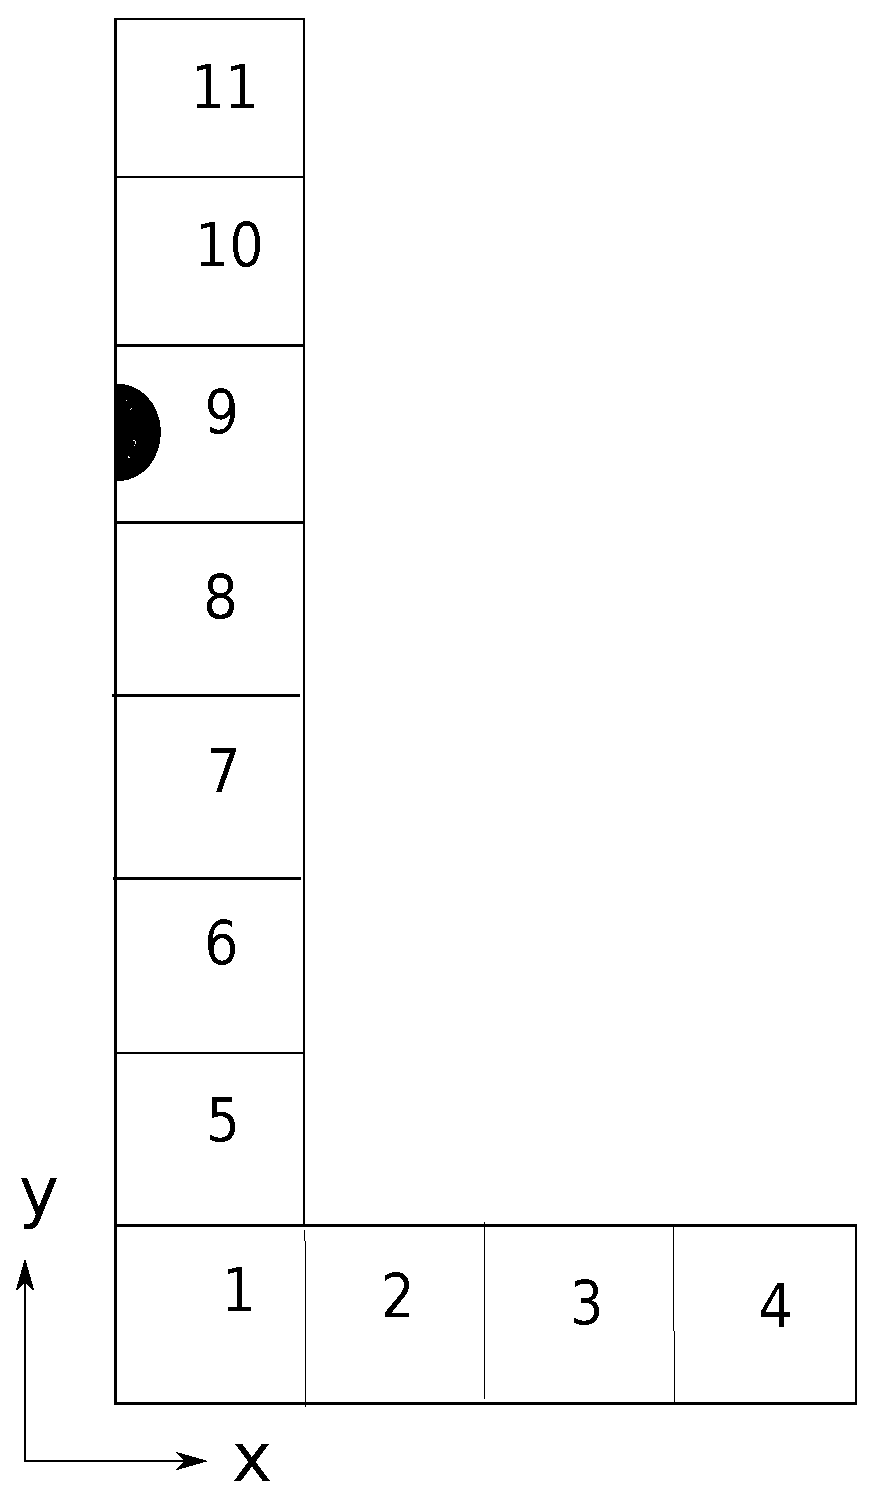
\includegraphics[scale = 0.5]{domain.eps}
 \caption{Domain for dimensional simulation}
\end{figure}
\subsection{Initial Condition}
Droplet Impact simulation is an initial value problem where initial condition determines the position of the drop in 
the domain. We have to specify the diameter of the droplet and the height of the center of droplet from the bottom of the 
first box of the domain.

\begin{equation}
 x^2+(y+(H_o-0.5L_b))^2D_{o}^{2}  %this equation is altered here from simulation there the axes are inverted
\end{equation}

\subsection{Boundary Conditions}
\begin{table}[H]
\centering
\begin{tabular}{||c c c c c||}
\hline
 Box ID & left & bottom & right & top  \\ 
 \hline\hline
 1 & free-slip & no-slip, SCA = $150^o$ & no-slip & no-slip  \\ 
 \hline
 2 & free-slip & no-slip, SCA = $150^o$ & no-slip & no-slip  \\ 
 \hline
 3 & free-slip & no-slip, SCA = $150^o$ & no-slip & no-slip  \\ 
 \hline
\end{tabular}
 \caption{Boundary conditions for domain}
\end{table}

\section{Non-Dimensional Simulations}

To run simulations in Non-Dimensionaly we have to find the non dimensional parameters for our problem.
We use Buckingham $\pi$ method to find out number of non dimensional parameters.
\begin{table}[H]
\centering
\caption{Dimensional matrix to determine non-dimensional groups}
\begin{tabular}{||c c c c c c c c c c||}
 \hline
 Dimensional Variables & $\rho_L$ & $\rho_g$ & $\mu_L$ & $\mu_g$ & $\sigma_{Lg}$ & $L_b$ & $D_o$ & $H_o$ & $g$ \\
 \hline\hline
 M & 1 & 1 & 1 & 1 & 1 & 0 & 0 & 0 & 0 \\
 \hline
 L & -3 & -3 & -1 & -1 & 0 & 1 & 1 & 1 & 1\\
 \hline
 T & 0 & 0 & -1 & -1& -2 & 0 & 0 & 0 & -2 \\
 \hline
\end{tabular}
\end{table}

Rank of the matrix = 3 \\

Number of independent non-dimensional parameters = 9-3 = 6 \\
\subsection{Domain}
\begin{figure}[H]
 \centering
 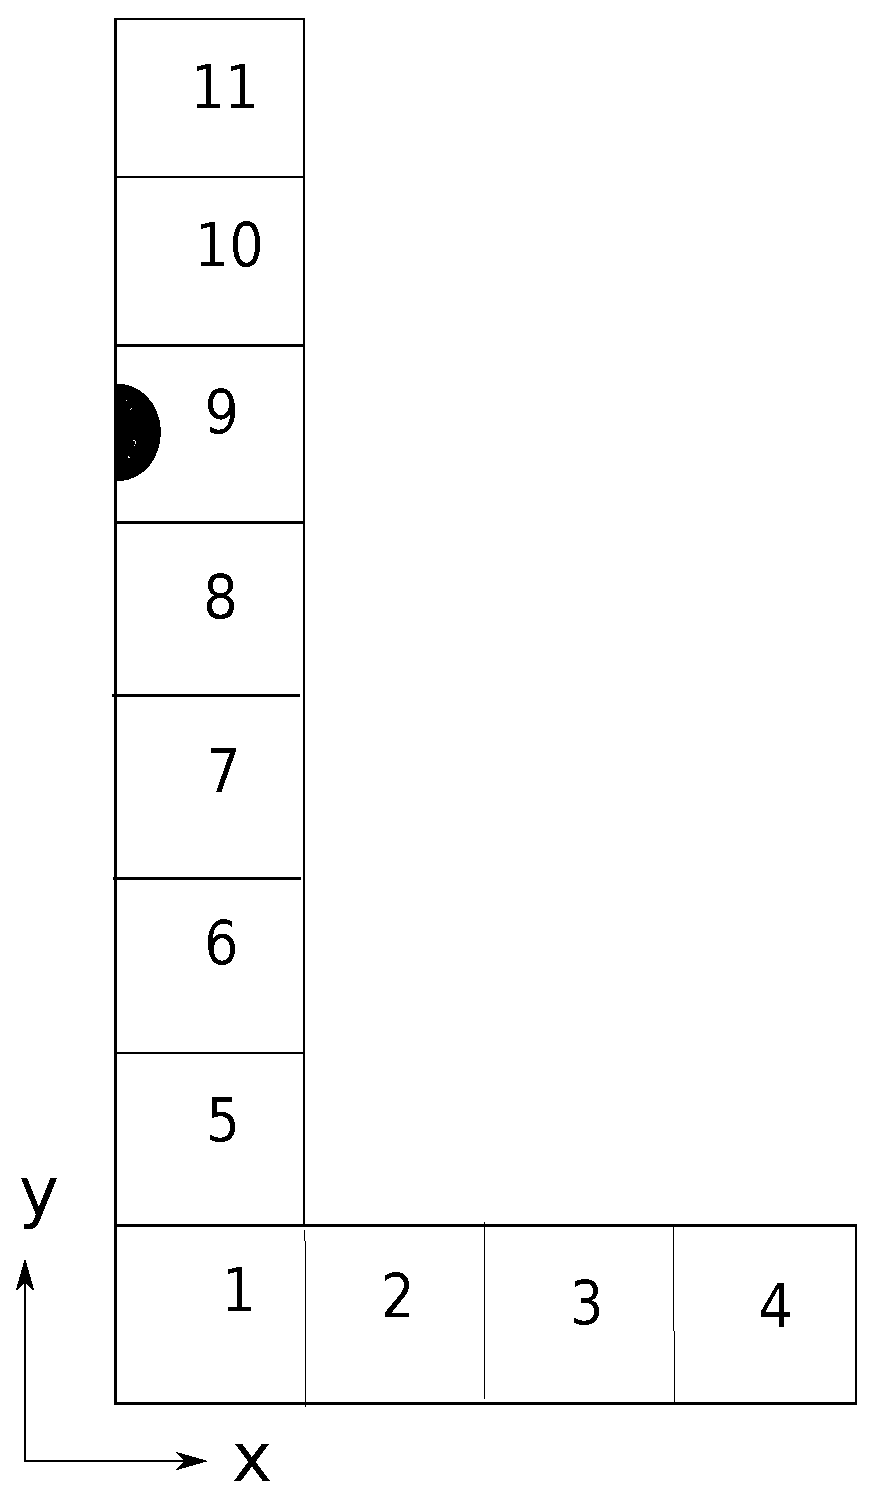
\includegraphics[scale=0.2]{domain}
 \caption{Domain for non-dimensional simulation}
\end{figure}

\subsection{Input to solver}
\begin{table}[H]
\centering
 \caption{Input for a multiphase solver in non-dimensional simulation}
\begin{tabular}{||c c c||}
\hline
 Parameter & Remark & Value  \\ 
 \hline\hline
 Re & Reynolds number & 2521.285386 \\
\hline
 We & Weber number of Liquid-gas & 29.43 \\
 \hline
 $H_k$ & $\frac{H_o}{D_o}$ &  12.00\\
 \hline
 $L_k$ & $\frac{L_o}{D_o}$ &  2 \\
 \hline
 $\rho_k$ & $\frac{\rho_g}{\rho_L}$ & $2 X 10^{-3}$  \\ 
 \hline
 $\mu_k$ & $\frac{\mu_g}{\mu_L}$ & $2 X 10^{-2}$ \\
 \hline
 \end{tabular}
 \end{table}


\subsection{Initial Condition}
The initial condition here is different from the dimensional simulation and compensates the differences in the governing
equations in both the simulations.
\begin{equation}
 x^2+(y+(H_k-0.5L_k))^2=0.25  %this equation is altered here from simulation there the axes are inverted
\end{equation}

\subsection{Boundary Conditions}
\begin{table}[H]
\centering
\caption{Boundary conditions for domain}
\begin{tabular}{||c c c c c||}
\hline
 Box ID & left & bottom & right & top  \\ 
 \hline\hline
 1 & - & no slip, SCA = $96^o$ & - & -  \\ 
 \hline
 2 & - & no slip, SCA = $96^o$ & - & outflow  \\ 
 \hline
 3 & - & no slip, SCA = $96^o$ & - & outflow  \\ 
 \hline
 4 & - & no slip, SCA = $96^o$ & outflow & outflow  \\ 
 \hline
 5 & - & - & outflow & -  \\ 
 \hline
\end{tabular}
\end{table}
\pagebreak
